\documentclass[lettersize,journal]{IEEEtran}
\usepackage{amsmath,amsfonts}
\usepackage{algorithmic}
\usepackage{algorithm}
\usepackage{array}
\usepackage[caption=false,font=normalsize,labelfont=sf,textfont=sf]{subfig}
\usepackage{textcomp}
\usepackage{stfloats}
\usepackage{url}
\usepackage{subfig}  
\usepackage{subcaption} 
\usepackage{verbatim}
\usepackage{graphicx}
\usepackage{cite}
\hyphenation{op-tical net-works semi-conduc-tor IEEE-Xplore}
% updated with editorial comments 8/9/2021

\begin{document}

\title{Self-Reproducing Robot: Concept Construction}

\author{Sylvester Zhang, Hod Lipson

\thanks{Sylvester Zhang is with the Department of Mechanical Engineering, Columbia University, New York, NY, USA (e-mail: sz3297@columbia.edu).

Hod Lipson is with the Department of Mechanical Engineering, Columbia University, New York, NY, USA (e-mail: hod.lipson@columbia.edu).}%
}

% Remember, if you use this you must call \IEEEpubidadjcol in the second
% column for its text to clear the IEEEpubid mark.

\maketitle

\begin{abstract}
Self-reproduction is a foundational principle in biological systems, offering a path toward scalable and autonomous construction in engineered environments. Here, we present a conceptual framework for a modular self-reproducing robot designed for operation in extreme or inaccessible conditions where human intervention is limited or infeasible. Inspired by cellular division, the system comprises identical modules capable of magnetic connection, disconnection, and reconfiguration through hinge-aligned stacking mechanisms. This architecture enables smooth, continuous 3D transformations and recursive structural replication with multiple degrees of freedom, including DNA-like configurations. The proposed design supports dynamic reassembly and structural scalability, laying the groundwork for autonomous robotic systems capable of adaptive growth. Future work will focus on hardware prototyping, learning-based simulation in MuJoCo, structural complexity analysis, and sim-to-real transfer, aiming to systematically explore the feasibility of this biologically inspired strategy and to establish a theoretical foundation for future applications in space and other high-risk environments.
\end{abstract}

\begin{IEEEkeywords}
Self-Reproducing Robot, Modules, Magnetic Control.
\end{IEEEkeywords}

\section{Introduction}
\IEEEPARstart{R}{obotic} systems have demonstrated remarkable utility across a wide range of structured environments, yet their deployment in remote, harsh, or unpredictable settings remains a major challenge. Applications such as space exploration\cite{you2025construction}, deep-sea inspection\cite{An_Overview_of_Robotics_and_Autonomous_Systems_for_Harsh_Environments}, and disaster response expose robots to operational conditions that are difficult to predict, maintain, or recover from. Over time, these conditions can lead to mechanical degradation, system failure, and mission interruption. Representative examples of such scenarios are illustrated in Fig.~\ref{fig:robotic_scenarios}, showcasing robotics in space, underwater, and post-disaster environments.
\begin{figure}[H]
    \centering
    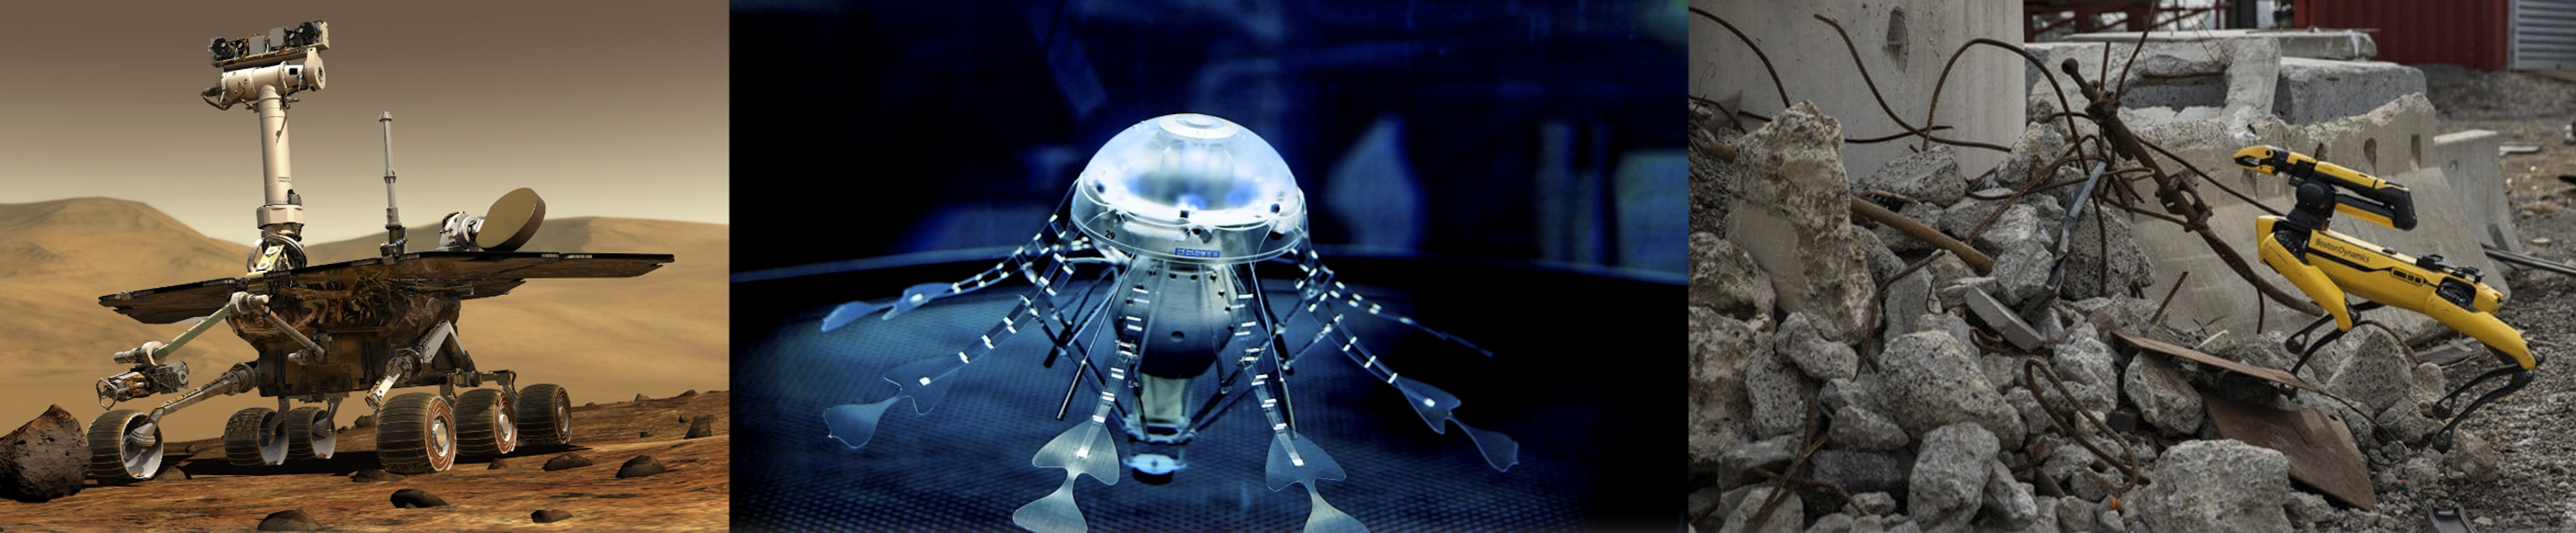
\includegraphics[width=1\linewidth]{extreme environment robot.png}
    \caption{Robots in extreme environments: (left) Mars rover from NASA, (middle) a bio-inspired underwater robot (source: Festo), and (right) Boston Dynamics' Spot for disaster response. Images sourced from the public internet and used here for educational purposes only.}
    \label{fig:robotic_scenarios}
\end{figure}

A key limitation of most engineered systems is their static nature. Once deployed, they lack the capacity to grow, repair, or reproduce\cite{4141032}. In contrast, biological systems offer a robust paradigm for sustainability. Cells, as shown in Fig.~\ref{cell division}, for example, reproduce through a cycle of absorbing external nutrients, expanding and dividing into identical offspring\cite{XU2016516}. This process enables autonomous propagation and resilience in changing environments.
\begin{figure}
    \centering
    \includegraphics[width=0.85\linewidth]{cell division.png}
    \caption{Illustration of the biological cell division process.}
    \label{cell division}
\end{figure}
Inspired by this biological principle\cite{doi:10.1073/pnas.1017075108}, the concept of a self-reproducing robot has emerged—one that can absorb modular components from its surroundings, expand its own structure, and assemble a detached copy of itself. Prior work in this area has primarily focused on three-dimensional modular architectures\cite{AbdelRahman2022}, such as cubic self-replicating robots\cite{zykoy2005self}. While effective in demonstrating feasibility, these systems often lack structural versatility and topological adaptability.

\begin{figure}[H]
    \centering
    \includegraphics[width=0.85\linewidth]{transformation from 2d to 3d.png}
    \caption{Reversible transformation between 2D and 3D.}
    \label{fig:2d to 3d}
\end{figure}
In this work, we introduce a planar-to-spatial self-reproducing robot composed of triangular modules connected via hinge joints. This design allows for reversible transformation between compact 2D configurations and functional 3D structures, as illustrated in Fig.~\ref{fig:2d to 3d}. By enabling foldable, stackable replication processes with multiple degrees of freedom, the system expands the geometric and operational scope of modular self-reproduction. This approach offers a new pathway to investigate the feasibility and structural mechanisms of biologically inspired robotic self-replication.

The remainder of this paper is organized as follows: Section II describes the detail concept construction; Section III concludes with future work; and Section IV for conclusion.

\section{Concept Construction}
Our proposed self-reproducing robot is composed of modular units that are capable of folding and autonomously attaching to each other through magnet. With magnet in each modules, as shown in Fig.~\ref{fig:folding}, they can connect together and become a huge one. Each piece is geometrically identical and designed to serve both as a structural component and as a reproductive element. This dual function allows the system to dynamically reconfigure itself and scale in structure through physical reproduction.

\begin{figure}[H]
    \centering
    \includegraphics[width=0.7\linewidth]{folding.png}
    \caption{Modular self-assembly process. Each triangular module can fold and unfold. With magnet in each modules, they can connect together and become a huge one. This forms the foundation of scalable physical self-reproduction.}
    \label{fig:folding}
\end{figure}

\subsection{Magnetically Controlled Connection Strategy}
At the center of this robot's design is a simple idea: using magnet force to control whether parts stick together or come apart. The robot doesn’t use complicated locks or motors to connect modules—instead, it changes the angle between parts by servo. I propose a mechanism based on angle-distance magnetic control, as shown in Fig.~\ref{fig:connection-desconnection}:
\begin{itemize}
    \item Decreasing the joint angle between two modules shortens the physical distance between embedded magnets, increasing magnetic force and triggering attachment.
    \item Increasing the angle causes the magnets to separate, weakening the force and allowing detachment.
\end{itemize}
\begin{figure}[H]
    \centering
    \includegraphics[width=0.7\linewidth]{connection-desconnection.png}
    \caption{Angle-Distance magnetic control between connection and disconnection.}
    \label{fig:connection-desconnection}
\end{figure}
And I come up with 2 versions of module to demonstrate.

\begin{figure}[H]
    \centering
    \includegraphics[width=0.5\linewidth]{version1module.png}
    \caption{Symmetric 4-Magnet module.}
    \label{fig:version1}
\end{figure}

\subsection{Version 1: Symmetric 4-Magnet Module}
The first version consists of modules with two magnets per piece, arranged symmetrically around a central hinge. Each completed module contains four magnets and one hinge, as shown in Fig.~\ref{fig:version1}, allowing it to bend and attach on both parts. We explored multiple configurations by stacking and pivoting these modules, illustrated in Fig.~\ref{fig:Modules Assemble into Various Structures}:
\begin{figure}[H]
    \centering
    \includegraphics[width=0.8\linewidth]{Modules Assemble into Various Structures.png}
    \caption{Modules assemble into various configurations.}
    \label{fig:Modules Assemble into Various Structures}
\end{figure}

\begin{itemize}
    \item When all hinges are placed on one side, the assembled structure behaves similarly to a continuum soft robot in Fig.~\ref{fig:Flexible bending enabled by simple stacking}, capable of smooth, nearly 360° bending.

\begin{figure}[H]
    \centering
    \includegraphics[width=0.5\linewidth]{bend 360.png}
    \caption{Flexible bending enabled by simple stacking.}
    \label{fig:Flexible bending enabled by simple stacking}
\end{figure}

    \item These modules can form a wide range of geometries—linear chains, branching trees, and looped clusters—demonstrating strong topological scalability and spatial flexibility in Fig.~\ref{fig:Modules Assemble into Various Structures}.

\begin{figure}[H]
  \centering

  \begin{minipage}[b]{0.4\linewidth}
    \centering
    \includegraphics[width=\linewidth]{13_7.png}
    \caption*{(a) Intermediate State}
  \end{minipage}
  \hfill
  \begin{minipage}[b]{0.5\linewidth}
    \centering
    \includegraphics[width=\linewidth]{10_10.png}
    \caption*{(b) Final Reproducing State}
  \end{minipage}

  \caption{Overall view of the Self-Reproduction process.}
  \label{fig:combined}
\end{figure}

\end{itemize}

Fig.~\ref{fig:combined} is the self-reproduction process. The left figure shows an intermediate state: the original robot enlarges itself by absorbing environmental modules while constructing a new robot; and the right figure shows the final state: the original robot has successfully generated a mirrored new individual through self-reproduction. With each robot consists of 10 modules.

\subsection{Version 2: Symmetric 6-Magnet Module}

To address the directional limitations observed in Version 1—where the placement of magnets restricted connectivity to certain orientations, I developed an enhanced module design that incorporates one hinge and six spherical magnets per unit. This configuration enables omnidirectional connection, allowing modules to attach along any axis without geometric conflict.

Each color-coded set consists of three modules, oriented in red, green, and blue directions respectively. These orientations are defined by the placement of a single hinge in each module, and due to the inherent symmetry of the triangular geometry, the direction angles between modules are separated by 120 degrees. This arrangement in Fig.~\ref{fig:Rotation about Different Directions} distributes the connection axes evenly in 3D space and ensures spatial uniformity during stacking or motion.

\begin{figure}[H]
    \centering
    \includegraphics[width=1\linewidth]{Rotation about Different Directions.png}
    \caption{Rotation about different directions.}
    \label{fig:Rotation about Different Directions}
\end{figure}

When simply stacked into a vertical structure composed of 15 such modules, the system achieves six degrees of freedom (6-DOF) in motion in Fig.~\ref{fig:6dof}, offering volumetric reconfigurability and highly flexible motion planning across 3D space.

\begin{figure}[H]
    \centering
    \includegraphics[width=1\linewidth]{6dof.png}
    \caption{Achieves 6 degrees of freedom (6 DOF) in motion.}
    \label{fig:6dof}
\end{figure}

This design significantly increases reproduction flexibility, as modules can now align, connect, and form nested structures in 3D space without external assistance.

\subsection{Emergent Helical Geometry and Bio-Inspired Possibilities}
During the expansion process, we observed an intriguing phenomenon in Fig.~\ref{fig:dna}: the modules, when stacked in certain orientations, tend to form a helical structure that visually resembles the double helix of DNA. While this geometric emergence was not explicitly designed, it raises interesting questions:

\begin{itemize}
    \item Could this structure offer mechanical benefits such as compliance, self-locking, or stability?
    \item Might the distributed twist and interleaved configuration contribute to robustness in uncertain environments?
\end{itemize}


\begin{figure}[H]
    \centering
    \includegraphics[width=1\linewidth]{dna.png}
    \caption{DNA-like structure.}
    \label{fig:dna}
\end{figure}

These possibilities are currently under preliminary observation, and we are actively exploring whether such naturally emerging forms might be harnessed as functional, bio-inspired design principles for future structural adaptation.

\subsection{Real-World Implementation Pathway}
The current prototype roadmap involves constructing each module with:
\begin{itemize}
    \item A servo motor for hinge actuation.
    \item Neodymium magnets for attachment.
    \item An onboard battery and IMU (Inertial Measurement Unit) for control and sensing.
    \item A microcontroller to execute reproduction logic.
\end{itemize}

Fig.~\ref{fig:evolution} illustrates the transformation of the system from a single modular unit to increasingly complex self-assembled structures, showcasing its inherent modularity and capacity for structural scaling. This progression reflects not only the ability of individual robots to grow by incorporating additional modules, but also the underlying design principles that support recursive assembly.

This growth process is inspired by biological evolution, where complexity arises from simple units through gradual adaptation. By applying this idea to hardware, the system suggests potential for adaptive structures that could evolve over generations. While current replication is deterministic, the framework hints at future integration of variation and feedback, enabling evolution-like behavior in physical robots.

\begin{figure}[H]
    \centering
    \includegraphics[width=0.94\linewidth]{evolution.png}
    \caption{Evolution of modular structures from a single unit to complex self-assembled forms, demonstrating scalability and bio-inspired growth potential.}
    \label{fig:evolution}
\end{figure}

\section{Future Work}

 My future work will focus on bridging the current conceptual design with real-world implementation and generalizing the system's self-reproduction capability. The first step involves constructing physical prototypes to experimentally validate the self-reproduction mechanism under real-world conditions. In parallel, we plan to build a simulation environment in MuJoCo, using learning algorithms to train autonomous self-reproduction behaviors.

 The planned research pipeline is summarized in Fig.~\ref{fig:pipeline}, outlining the key stages from concept validation to full system deployment.

Another important direction is the exploration of structural complexity, investigating how variations in modular configurations impact the system’s robustness, adaptability, and efficiency. Insights from these simulations will support the development of sim-to-real transfer techniques, enabling policies trained in virtual environments to be deployed reliably on physical hardware.

\begin{figure}[H]
    \centering
    \includegraphics[width=0.65\linewidth]{pipeline.png}
    \caption{Work Pipeline}
    \label{fig:pipeline}
\end{figure}

\section{Conclusion}
This work presents a biologically inspired framework for modular self-reproducing robots, demonstrating scalable assembly and transformation in concept construction. Future research will aim to realize real-world prototype development and explore adaptive structural evolution.


\section*{Acknowledgments}
The author would like to express his gratitude to Professor Hod Lipson for his invaluable guidance and support throughout this project. 

\bibliographystyle{IEEEtran}  
\bibliography{reference}  


%\newpage


 
% \vspace{11pt}

\begin{IEEEbiography}[{\includegraphics[width=1in,height=1.25in,clip,keepaspectratio]{IEEE-Transactions-LaTeX2e-templates-and-instructions/my photo.jpeg}}]{Sylvester Zhang}
 received the B.E. degree in Aeronautical and Astronautical Engineering from Sun Yat-sen University, Shenzhen, China, 2024. And currently he is working toward the M.S. degree in Robotics concentration of Mechanical Engineering with Columbia University. His research interests include Soft Manipulator, Bio-inspired Robotics and  Self-Reproducing Robot.
\end{IEEEbiography}




\vfill

\end{document}


